\documentclass[10pt,a4paper]{article}
\usepackage[margin=1.6cm,top=1.3cm,bottom=1.4cm]{geometry}
\usepackage{graphicx,booktabs,amsmath,amssymb,xcolor,float}
\usepackage[font=small,labelfont=bf,skip=2pt]{caption}
\usepackage[compact]{titlesec}
\usepackage{enumitem}
\usepackage[hidelinks]{hyperref}
\usepackage{tikz}
\usetikzlibrary{arrows.meta,positioning,calc,fit}
\usepackage{capt-of}
\usepackage{multirow}

\titlespacing*{\section}{0pt}{5pt}{2pt}
\titlespacing*{\subsection}{0pt}{4pt}{1pt}
\titleformat{\section}{\normalfont\large\bfseries}{}{0em}{}
\titleformat{\subsection}{\normalfont\normalsize\bfseries}{}{0em}{}
\setlist[itemize]{leftmargin=1.1em,itemsep=0.5pt,topsep=1pt,parsep=0pt}
\setlength{\parskip}{1.2pt}
\setlength{\abovedisplayskip}{3pt}
\setlength{\belowdisplayskip}{3pt}
\setlength{\textfloatsep}{5pt}
\setlength{\intextsep}{4pt}
\renewcommand{\arraystretch}{0.95}
\captionsetup[table]{skip=1pt}
\newcommand{\D}{\mathcal{D}}

\begin{document}
\pagestyle{plain}

\begin{center}
{\Large\bfseries COMP6010 Assignment: From Bayesian Inference to Generative AI}\\[2pt]
{\normalsize Planning and Handling Uncertainty in Machine Learning}\\[3pt]
{\bfseries Satria Pamungkas} \quad\textbullet\quad Student ID: {\bfseries 21522611}
\quad\textbullet\quad Part C option: {\bfseries C2} (animal drawings, flow matching)\\[2pt]
{\small Supplement: \texttt{Satria\_Pamungkas\_21522611\_COMP6010\_Supplement.zip}}
\end{center}
\vspace{-4pt}
\hrule
\vspace{3pt}

\noindent\textbf{Introduction.}
This report answers three connected questions with one method: probability. Part~A performs
\emph{inference} in a fully known five-variable Bayesian network, where the difficulty is
conditioning on evidence correctly. Part~B \emph{learns} a single unknown parameter and shows why a
decision must be driven by the whole posterior rather than a point estimate. Part~C \emph{learns a
generative model} --- a conditional flow-matching network trained from scratch on Quick, Draw!
animal drawings --- and shows that the same factorise/learn/sample pattern scales from five binary
variables to images. Every number cited is produced by the notebooks in the supplement and stored in
a named CSV or JSON file; file names appear in \textcolor{gray}{\small\texttt{grey monospace}}.

\section{Part A: Bayesian-network simulation and sampling inference}

\subsection{A1. Model, factorisation and exact reference values}

The five binary variables are $H$ (hot weather), $F$ (irrigation fault), $D$ (dry soil), $S$ (sensor
reports ``dry''), $W$ (plants wilting), with edges $H\!\to\!D$, $F\!\to\!D$, $D\!\to\!S$,
$D\!\to\!W$, $H\!\to\!W$ and independent roots $P(H{=}1)=0.30$, $P(F{=}1)=0.08$.

\begin{minipage}[t]{0.30\textwidth}
\vspace{2pt}
\centering
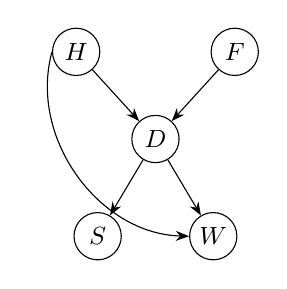
\begin{tikzpicture}[>=Stealth,node distance=9mm and 9mm,
  every node/.style={circle,draw,minimum size=6.0mm,inner sep=0pt,font=\small}]
\node (H) {$H$};
\node (F) [right=14mm of H] {$F$};
\node (D) [below=8mm of $(H)!0.5!(F)$] {$D$};
\node (S) [below left=8mm and 3mm of D] {$S$};
\node (W) [below right=8mm and 3mm of D] {$W$};
\draw[->] (H) -- (D); \draw[->] (F) -- (D);
\draw[->] (D) -- (S); \draw[->] (D) -- (W);
\draw[->] (H.west) to[bend right=52] (W.west);
\end{tikzpicture}
\end{minipage}%
\begin{minipage}[t]{0.68\textwidth}
\vspace{4pt}
The graph gives the factorisation
\[
P(H,F,D,S,W)=P(H)\,P(F)\,P(D\mid H,F)\,P(S\mid D)\,P(W\mid H,D),
\]
i.e.\ $2{+}2{+}4{+}2{+}4$ CPT entries rather than the 31 free parameters of an unconstrained joint.
One implied conditional independence is $\;S \perp W \mid D,H\;$: $S$ depends on the network only
through its single parent $D$, so once $D$ (and $H$, which also parents $W$) is fixed, the sensor
reading says nothing further about wilting. Verified numerically to
$\max|P(S\mid D,H,W)-P(S\mid D,H)| < 10^{-16}$.
\end{minipage}

\smallskip
Enumerating all $2^5=32$ states gives $\sum P = 1$ to within $2\times10^{-16}$ and the exact
references in Table~\ref{tab:Aexact}. Two further checks matter. First, marginalising recovers
$P(H{=}1)=0.30$ and $P(F{=}1)=0.08$, and $P(H{=}1,F{=}1)=P(H{=}1)P(F{=}1)$ confirms prior root
independence. Second, and more usefully, I deliberately transposed the $H,F$ indices in the $D$
lookup: the joint \emph{still} summed to $1$, so a normalisation test alone would not have caught
the bug, whereas the query values changed visibly ($q_1$ became $0.2044$). A passing normalisation
check is necessary but far from sufficient.
\textcolor{gray}{\small\texttt{A1\_exact\_reference\_values.csv}, \texttt{A1\_joint\_enumeration\_32\_states.csv}}

\begin{table}[H]\centering\small
\caption{Exact values by enumeration, with the evidence probability that governs rejection-sampling efficiency.}
\label{tab:Aexact}
\begin{tabular}{llrrr}
\toprule
Query & Definition & Exact value & $P(\text{evidence})$ & Retained per 1{,}000 \\
\midrule
$q_1$ & $P(F{=}1\mid S{=}1)$ & 0.231504 & 0.26816 & 268 \\
$q_2$ & $P(F{=}1\mid S{=}1,W{=}1)$ & 0.293294 & 0.15932 & 159 \\
$q_3$ & $P(F{=}1\mid S{=}1,W{=}1,H{=}1)$ & 0.168675 & 0.10956 & 110 \\
\bottomrule
\end{tabular}
\end{table}

\subsection{A2. Forward sampling and rejection-based inference}

To sample a binary $X$ with $P(X{=}1\mid\text{pa})=p$, draw $u\sim\mathrm{Uniform}[0,1)$ and set
$x=\mathbb{1}[u<p]$; since the uniform CDF is $F(u)=u$, we get $P(x{=}1)=P(u<p)=p$ exactly. This is
inverse-CDF sampling with the unit interval cut at $p$, so the two sub-interval widths \emph{are}
the two probabilities. The correct CPT row is selected using the already-sampled parent values,
which is why the loop must follow the topological order $(H,F,D,S,W)$: every variable's parents are
assigned before it is drawn, and the resulting assignments are i.i.d.\ draws from the exact joint.

Rejection sampling then discards every sample inconsistent with the evidence $e$ and reports the
fraction of survivors with $F{=}1$; this is valid because conditioning on an event and restricting
to it are the same operation. Its cost is that the retained fraction is $P(e)$. I generate one joint
sample set per seed and reuse it for all three queries, at $N\in\{10^3,10^4,10^5\}$ with five seeds
each. Measured retained fractions match Table~\ref{tab:Aexact} closely (e.g.\ $0.1590$ against
$0.15932$ for $q_2$ at $N{=}10^5$). No estimate was undefined across the 45 runs --- the smallest
retained count was 107, for $q_3$ at $N{=}10^3$ --- but the $0/0$ case returns \texttt{NaN} rather
than an invented value, as required.
\textcolor{gray}{\small\texttt{A2\_rejection\_per\_run.csv}}

\subsection{A3. Likelihood weighting}

I implement likelihood weighting only (the brief warns against adding Gibbs merely to increase code
volume). Evidence variables are \emph{clamped}; the rest are sampled in topological order; each
sample is weighted by $w=\prod_{E_i\in\mathcal{E}}P(E_i{=}e_i\mid\mathrm{pa}(E_i))$, and

\vspace{-3pt}
\[
\hat P(F{=}1\mid e)=\frac{\sum_{k:F^{(k)}=1}w^{(k)}}{\sum_k w^{(k)}}.
\]

\textbf{Why weights are required.} Clamping draws from the mutilated network
$Q(x_{-\mathcal{E}})=\prod_{X_i\notin\mathcal{E}}P(x_i\mid\mathrm{pa}_i)$, not from the posterior.
Since $P(x_{-\mathcal{E}}\mid e)=Q(x_{-\mathcal{E}})\,w(x_{-\mathcal{E}})/P(e)$, the weight is
exactly the importance ratio, giving $\mathbb{E}_Q[w\,\mathbb{1}(F{=}1)]=P(F{=}1,e)$ and
$\mathbb{E}_Q[w]=P(e)$. Counting \emph{unweighted} would compute $Q(F{=}1)$, which here is just the
prior: I measured $0.0800$ against the exact $q_2=0.2933$, because clamping a \emph{descendant}
cannot change how its \emph{ancestors} were drawn. The weights are what carry evidence back up the
graph. Normalisation must use $\sum_k w^{(k)}$ (a Monte-Carlo estimate of $P(e)$; the mean weight
came to $0.1600$ against the exact $0.159316$) --- dividing by $N$ would return the joint
$P(F{=}1,e)$ instead. Note $H$ in $q_3$ is a \emph{root} evidence variable, so it contributes the
constant $0.30$; only non-root evidence makes weights vary.
\textcolor{gray}{\small\texttt{A3\_likelihood\_weighting\_per\_run.csv}}

\subsection{A4. Comparison and interpretation}

\begin{figure}[H]\centering
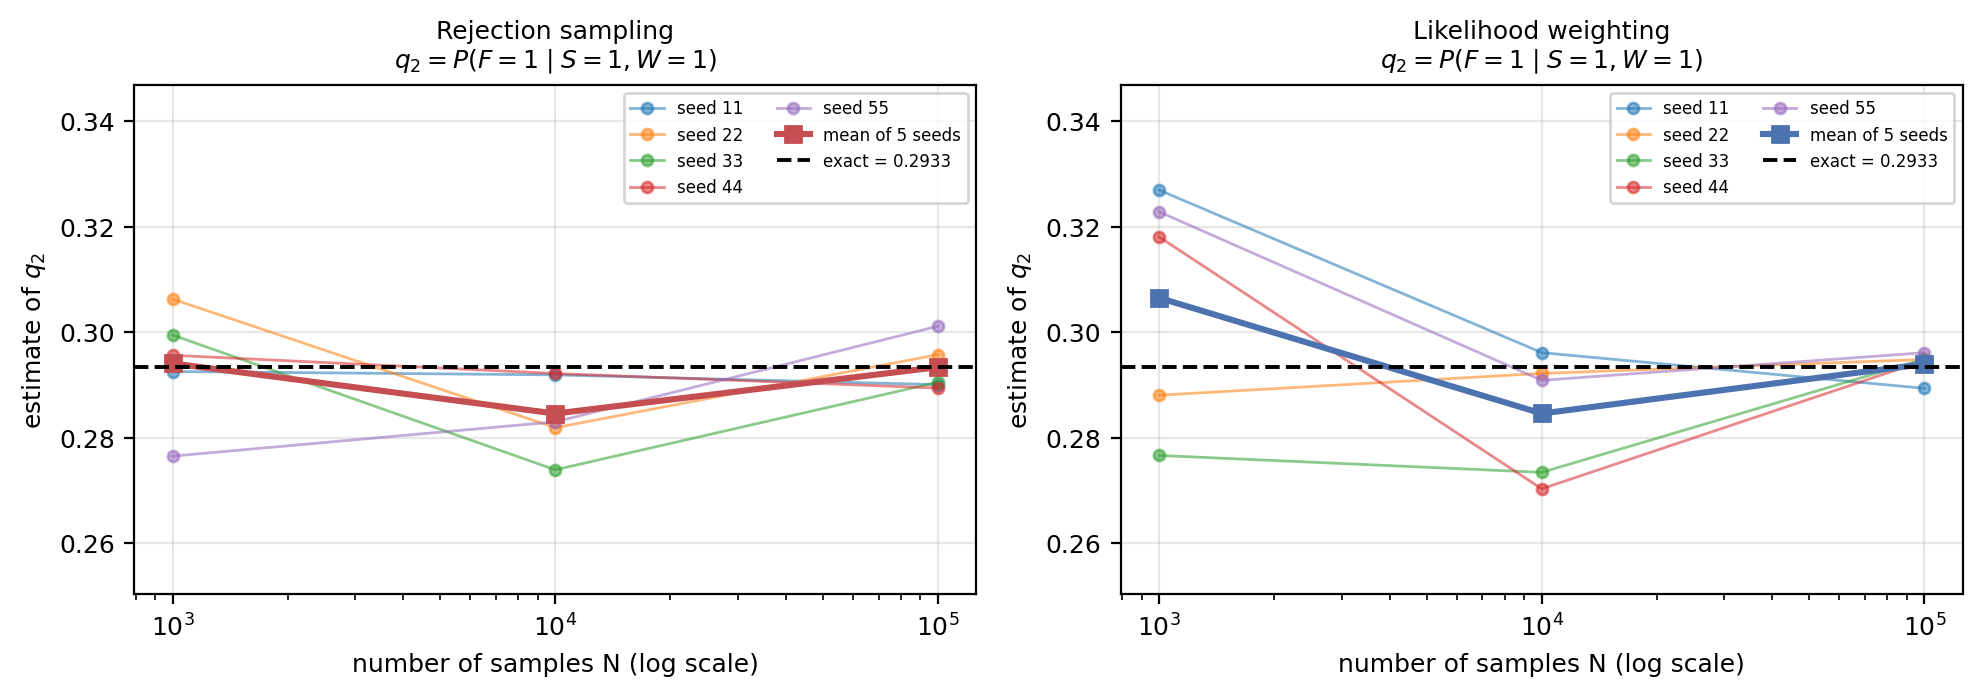
\includegraphics[width=0.62\textwidth]{../Satria_Pamungkas_21522611_COMP6010_Supplement/results/partA/A4_convergence_q2.png}
\hfill
\begin{minipage}[b]{0.36\textwidth}
\small
\captionof{table}{Mean $\pm$ sd over five seeds.}
\label{tab:Acmp}
\vspace{-3pt}
\begin{tabular}{@{}llll@{}}
\toprule
 & $N$ & Rejection & Lik.\ weight. \\
\midrule
$q_1$ & $10^3$ & .238$\pm$.014 & .251$\pm$.040 \\
      & $10^4$ & .228$\pm$.007 & .227$\pm$.009 \\
      & $10^5$ & .231$\pm$.003 & .231$\pm$.002 \\
$q_2$ & $10^3$ & .294$\pm$.011 & .307$\pm$.023 \\
      & $10^4$ & .285$\pm$.008 & .285$\pm$.012 \\
      & $10^5$ & .293$\pm$.005 & .294$\pm$.003 \\
$q_3$ & $10^3$ & .170$\pm$.019 & .173$\pm$.016 \\
      & $10^4$ & .161$\pm$.018 & .167$\pm$.004 \\
      & $10^5$ & .169$\pm$.005 & .169$\pm$.001 \\
\bottomrule
\end{tabular}
\end{minipage}
\caption{Convergence of $q_2$ (five seeds, exact value dashed). Both estimators are consistent;
spread narrows as $N^{-1/2}$. \textcolor{gray}{\small\texttt{A4\_convergence\_q2.png}, \texttt{A4\_summary\_table.csv}}}
\label{fig:Aconv}
\end{figure}

\textbf{Evidence accumulation.} Against the prior $P(F{=}1)=0.08$: a dry-soil alert raises the fault
probability to $q_1=0.2315$ ($2.9\times$ the prior) but leaves it low, because the sensor is only
90\% accurate and dry soil has a far more common competing cause (hot weather, prior $0.30$ versus
the fault's $0.08$). Adding wilting gives $q_2=0.2933$: $W$ is a \emph{second, independent} symptom
of dry soil, so it corroborates rather than repeats the sensor --- $S\perp W\mid D,H$ means they are
two separate measurements of the same hidden state. Adding hot weather \emph{reverses} the direction,
$q_3=0.1687$. This is \textbf{explaining away}: $D$ is a collider on $H\to D\leftarrow F$, so
confirming an alternative sufficient cause makes the fault less necessary. Practically, a dry-soil
alert on a hot day is much weaker evidence of a fault than the same alert on a cool day. These are
conditional probabilities under the supplied hypothetical model, not evidence of real-world
causation. \textcolor{gray}{\small\texttt{A4\_evidence\_sequence.csv}}

\textbf{Accuracy versus effort.} Rejection sampling keeps only the fraction $P(e)$ of its samples, so
each added evidence variable shrinks the usable set: at $N{=}10^5$ it retains ${\sim}26{,}800$
samples for $q_1$ but only ${\sim}10{,}900$ for $q_3$. Likelihood weighting retains all $N$. With the
five seeds the brief requires, this ordering is \emph{not} reliably visible --- rejection happens to
win some $q_1$/$q_2$ rows in Table~\ref{tab:Acmp} --- so I ran a supplementary 400-seed check:
likelihood weighting then has lower sd and lower MAE in \textbf{9 of 9} (query, $N$) combinations,
with a sd ratio of $1.04$--$1.26$ for $q_1$/$q_2$ and a consistent $2.05\times$ for $q_3$, the most
heavily conditioned query. That five seeds cannot rank two estimators whose variances differ by less
than a factor of two is itself the lesson. On weight concentration, the Kish effective sample size
$\mathrm{ESS}=(\sum w)^2/\sum w^2$ gives $\mathrm{ESS}/N$ of $0.40$, $0.22$ and $0.46$ for
$q_1,q_2,q_3$: the weight takes only a few distinct values here (discrete evidence CPT entries), the
top 1\% of weights hold under 6\% of total mass, so \emph{no} few samples dominate. That is a
property of this small network with mild evidence, not a general guarantee. One caveat on cost:
rejection generates one sample set reused by all three queries, whereas likelihood weighting must
re-run per evidence set, so I report their timings separately rather than equating a ``sample''
across methods. \textcolor{gray}{\small\texttt{A4\_variance\_check\_400seeds.csv}, \texttt{A4\_timing.csv}}

\textbf{Why more samples need not help every run.} Each estimate is a random variable; increasing $N$
reduces its \emph{variance}, so error falls on average and the seed spread narrows, but a single run
can be lucky at small $N$. Concretely, for $q_2$ under rejection sampling seeds 11 and 33 got
\emph{worse} from $N{=}10^3$ to $10^4$, and seeds 11 and 44 from $10^4$ to $10^5$. Only the
aggregated mean and sd are evidence about an estimator; a single run is not, which is exactly why
five seeds are required.

\textbf{Why fixing downstream evidence is invalid.} Forward sampling draws each variable from
$P(x_i\mid\mathrm{pa}_i)$, so influence flows only parent$\,\to\,$child. Overwriting an observed
descendant after the fact cannot change how its ancestors were drawn: doing this for $S{=}1,W{=}1$
over 200{,}000 samples returned $0.0799$ --- the prior --- instead of $q_2=0.2933$. Diagnostic
reasoning runs \emph{against} the arrows, so a correction is mandatory: either discard mismatching
samples (rejection) or re-weight by the evidence likelihood (likelihood weighting).

\section{Part B: Bayesian learning with a Beta prior}

\subsection{B1. Formulation}

Each grasp attempt succeeds or fails, so the Bernoulli distribution --- the only distribution on
$\{0,1\}$, with one parameter --- is the natural likelihood,
$P(X_i{=}x\mid\theta)=\theta^x(1-\theta)^{1-x}$. For $n$ conditionally independent attempts with $s$
successes the likelihood is $\theta^s(1-\theta)^{n-s}$, depending on the data only through the
sufficient statistics $(s,n)$. The parameter $\theta$ is not an outcome: it is an unknown
\emph{continuous} quantity in $(0,1)$, so uncertainty about it needs a density, and the Beta family
is supported exactly on $(0,1)$. The decisive property is \textbf{conjugacy}: the Beta kernel
$\theta^{\alpha-1}(1-\theta)^{\beta-1}$ has the same algebraic form as the likelihood, so the
posterior is again Beta and updating is exact arithmetic on two numbers. Here $\alpha,\beta$ are
\emph{prior shape parameters, not data}; they behave like $\alpha{-}1$ pseudo-successes and
$\beta{-}1$ pseudo-failures, so $\mathrm{Beta}(2,3)$ is a mildly pessimistic belief (mean $0.4$)
carrying about as much weight as three real attempts.

\begin{minipage}[t]{0.34\textwidth}
\vspace{1pt}
\centering
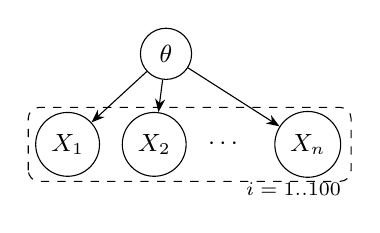
\begin{tikzpicture}[>=Stealth,font=\small]
\node[circle,draw,minimum size=6.5mm] (th) at (0,0) {$\theta$};
\node[circle,draw,minimum size=6mm] (x1) at (-1.25,-1.15) {$X_1$};
\node[circle,draw,minimum size=6mm] (x2) at (-0.15,-1.15) {$X_2$};
\node (dots) at (0.75,-1.15) {$\cdots$};
\node[circle,draw,minimum size=6mm] (xn) at (1.8,-1.15) {$X_{n}$};
\draw[->] (th) -- (x1); \draw[->] (th) -- (x2); \draw[->] (th) -- (xn);
\draw[dashed,rounded corners] (-1.75,-1.62) rectangle (2.35,-0.68);
\node[font=\scriptsize] at (1.62,-1.72) {$i=1..100$};
\end{tikzpicture}
\end{minipage}%
\begin{minipage}[t]{0.65\textwidth}
\vspace{4pt}
$\theta$ is the single shared parent of every observation, so
$f(\theta,x_1..x_n)=f(\theta)\prod_i P(x_i\mid\theta)$ and $X_i \perp X_j \mid \theta$: once $\theta$
is fixed, attempt 3's outcome says nothing about attempt 4. The $X_i$ are \emph{not} marginally
independent --- integrating $\theta$ out does not factorise. I verified this by simulation:
$P(X_2{=}1\mid X_1{=}1)=0.4283$ versus $P(X_2{=}1\mid X_1{=}0)=0.3335$ under the prior, but both equal
$0.55$ when $\theta$ is held fixed. This common-cause dependence is what \emph{makes learning
possible}: if attempts were marginally independent, data could not inform us about $\theta$.
Note also that a density is not a probability --- $f(0.8)$ may exceed 1, while $P(\theta{=}0.8)=0$
exactly, which is why B3 asks for a tail mass rather than a density value.
\end{minipage}

\subsection{B2. Posterior updating}

Substituting the Bernoulli likelihood and Beta prior into Bayes' rule and absorbing every
$\theta$-free factor into the normalising constant,
\[
f(\theta\mid\D)\;\propto\;\underbrace{\theta^{s}(1-\theta)^{n-s}}_{\text{likelihood}}\cdot
\underbrace{\theta^{\alpha-1}(1-\theta)^{\beta-1}}_{\text{prior}}
=\theta^{(\alpha+s)-1}(1-\theta)^{(\beta+n-s)-1}
\;\Longrightarrow\;
\theta\mid\D\sim\mathrm{Beta}(\alpha+s,\;\beta+n-s),
\]
so updating adds successes to $\alpha$ and failures to $\beta$. Sequential and pooled updating
\emph{must} agree, because the likelihood factorises across batches and multiplication is
order-independent; both give $\mathrm{Beta}(2{+}85,\,3{+}15)=\mathbf{Beta(87,18)}$ and the notebook
asserts the equality. I also checked the conjugate shortcut against brute-force numerical Bayes on a
200{,}001-point grid (max density difference ${\sim}10^{-9}$) and confirmed all six batch orderings
return the same posterior. \textcolor{gray}{\small\texttt{B2\_sequential\_updates.csv}}

\begin{table}[H]\centering\small
\caption{Cumulative point estimates. The three estimators converge as the prior's weight (${\sim}3$
pseudo-attempts) is swamped by data. \textcolor{gray}{\small\texttt{B2\_point\_estimates.csv}}}
\label{tab:Bpoint}
\begin{tabular}{lrrrrrr}
\toprule
Stage & Posterior & Cum.\ $n$ & Cum.\ $s$ & ML $s/n$ & Post.\ mean & MAP \\
\midrule
Prior & $\mathrm{Beta}(2,3)$ & 0 & 0 & --- & 0.4000 & 0.3333 \\
After batch 1 & $\mathrm{Beta}(8,7)$ & 10 & 6 & 0.6000 & 0.5333 & 0.5385 \\
After batch 2 & $\mathrm{Beta}(24,11)$ & 30 & 22 & 0.7333 & 0.6857 & 0.6970 \\
After batch 3 & $\mathrm{Beta}(87,18)$ & 100 & 85 & 0.8500 & \textbf{0.8286} & 0.8350 \\
\bottomrule
\end{tabular}
\end{table}

The gap $|$post.\ mean $-$ ML$|$ shrinks from $0.067$ after batch 1 to $0.021$ after batch 3: the
prior pulls hardest when data are scarce. MAP sits between ML and the posterior mean because the mode
of this left-skewed posterior lies above its mean.

\subsection{B3. Uncertainty and the deployment decision}

Three distinct quantities, all from $\mathrm{Beta}(87,18)$:

\textbf{(1) Posterior predictive.} We do not know $\theta$, so we average over the posterior rather
than plugging in an estimate:
$P(X_{n+1}{=}1\mid\D)=\int_0^1\theta\,f(\theta\mid\D)\,d\theta=\mathbb{E}[\theta\mid\D]=\alpha_n/(\alpha_n{+}\beta_n)=\mathbf{0.8286}$.
It \emph{numerically} equals the posterior mean, but the two are conceptually distinct --- one is
about a future observation, the other summarises a parameter distribution. The coincidence is a
property of the linear expectation and vanishes for anything non-linear: the probability that the next
\emph{two} attempts both succeed is $\mathbb{E}[\theta^2]=0.6879 > (\mathbb{E}[\theta])^2=0.6865$ by
Jensen's inequality, strictly above the plug-in answer.

\textbf{(2) 95\% equal-tailed credible interval:} $[\mathbf{0.7512},\,\mathbf{0.8941}]$ from the
posterior quantiles, verified by $F(\text{lo})=0.025$, $F(\text{hi})=0.975$.

\textbf{(3) Threshold mass:} $P(\theta>0.8\mid\D)=1-F(0.8)=\mathbf{0.7883}$, confirmed two ways ---
numerical integration gives $0.78826666$ against SciPy's $0.78826666$, and 200{,}000 posterior draws
(seed \texttt{20260910}) give $0.78688$, within $0.5$ standard errors of the analytic value.

\textbf{Decision: the rule is NOT met.} It requires $P(\theta>0.8\mid\D)\ge0.95$; the evidence gives
$0.7883$, a shortfall of $0.1617$. At the observed success rate, roughly 400--500 further attempts
would be needed to satisfy it.

\textbf{Why a point estimate above 0.8 is not sufficient.} Both ML $(0.8500)$ and the posterior mean
$(0.8286)$ lie \emph{above} the threshold, yet the rule still fails. A point estimate discards the
posterior's width. With 100 attempts the posterior retains real spread (sd $0.0366$) and 21.2\% of
its mass sits below $0.8$; the credible interval's lower bound, $0.7512$, is below the threshold, so
$\theta<0.8$ has not been ruled out. The rule is deliberately written about the whole distribution
because the cost of an unreliable gripper is incurred when $\theta$ is genuinely low, not when the
average looks acceptable. Passing requires the posterior to be \emph{concentrated} above $0.8$.

\textbf{Why a PDF value at 0.8 is not this probability.} $f(0.8)=7.26$ is a density --- a
probability-per-unit-$\theta$ --- and cannot be compared with $0.95$ at all; this posterior peaks at
$10.96$, well above 1. A single point has probability exactly zero for a continuous parameter. The rule
needs the \emph{area} $\int_{0.8}^{1}f(\theta\mid\D)\,d\theta$. The notebook verifies the relationship
directly: $P(0.8\pm0.0005)=0.0072565$ against $f(0.8)\times0.001=0.0072556$, which is what a density
means. \textcolor{gray}{\small\texttt{B3\_decision.json}, \texttt{B3\_mc\_verification.png}}

\begin{figure}[H]\centering
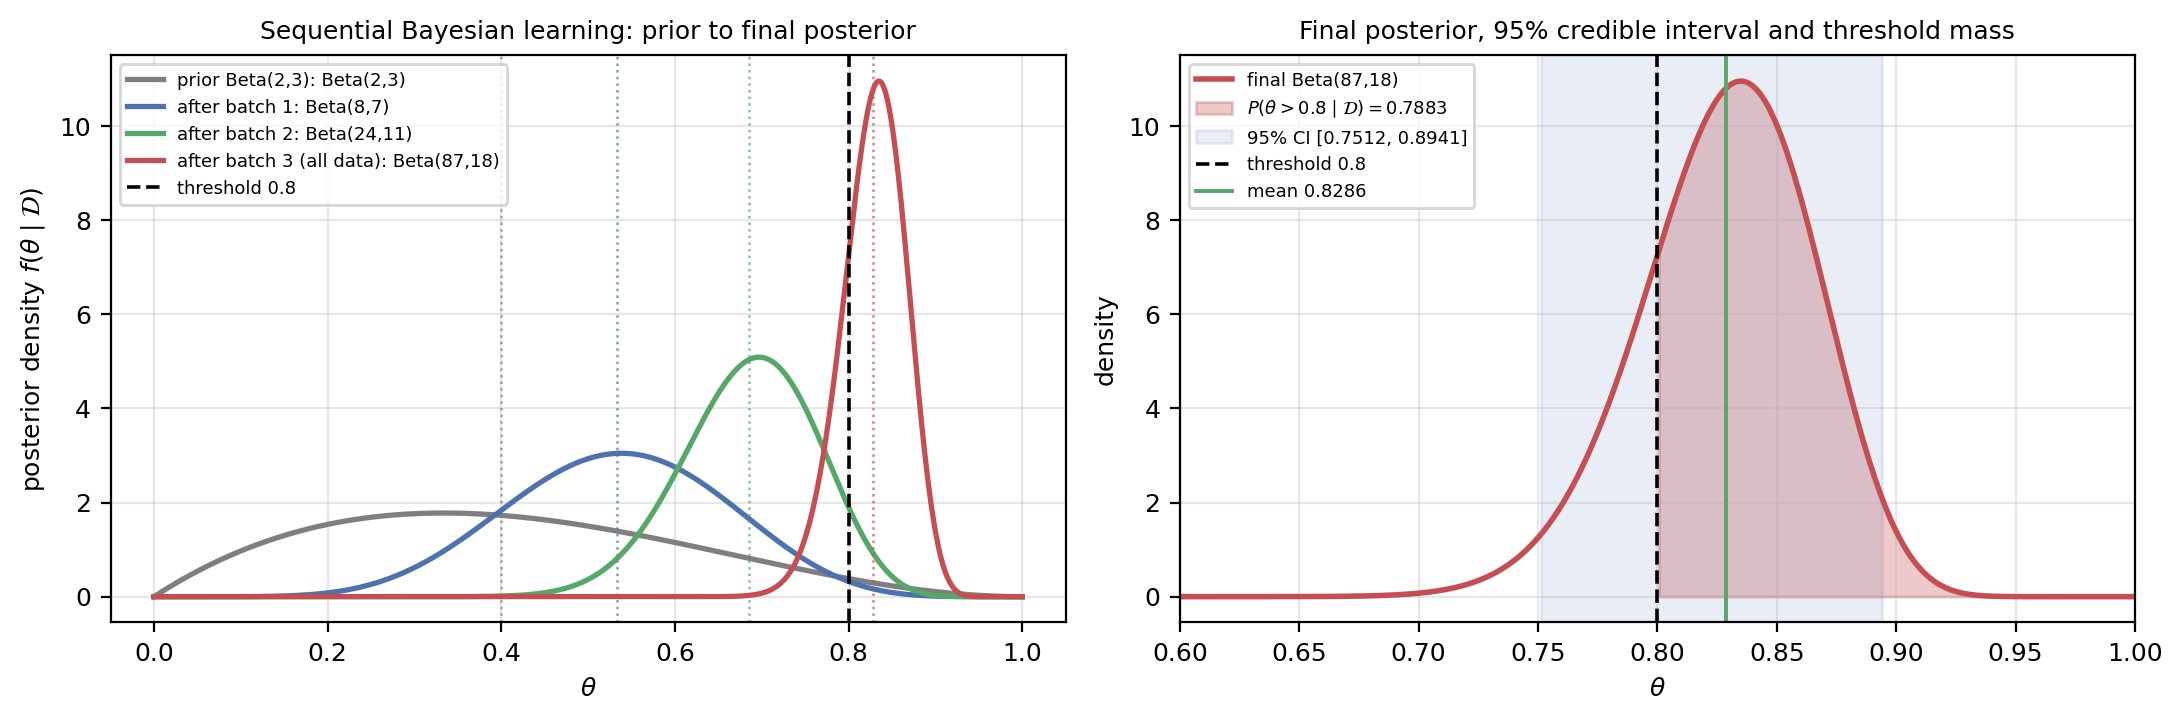
\includegraphics[width=0.495\textwidth]{../Satria_Pamungkas_21522611_COMP6010_Supplement/results/partB/B2_posterior_evolution.png}
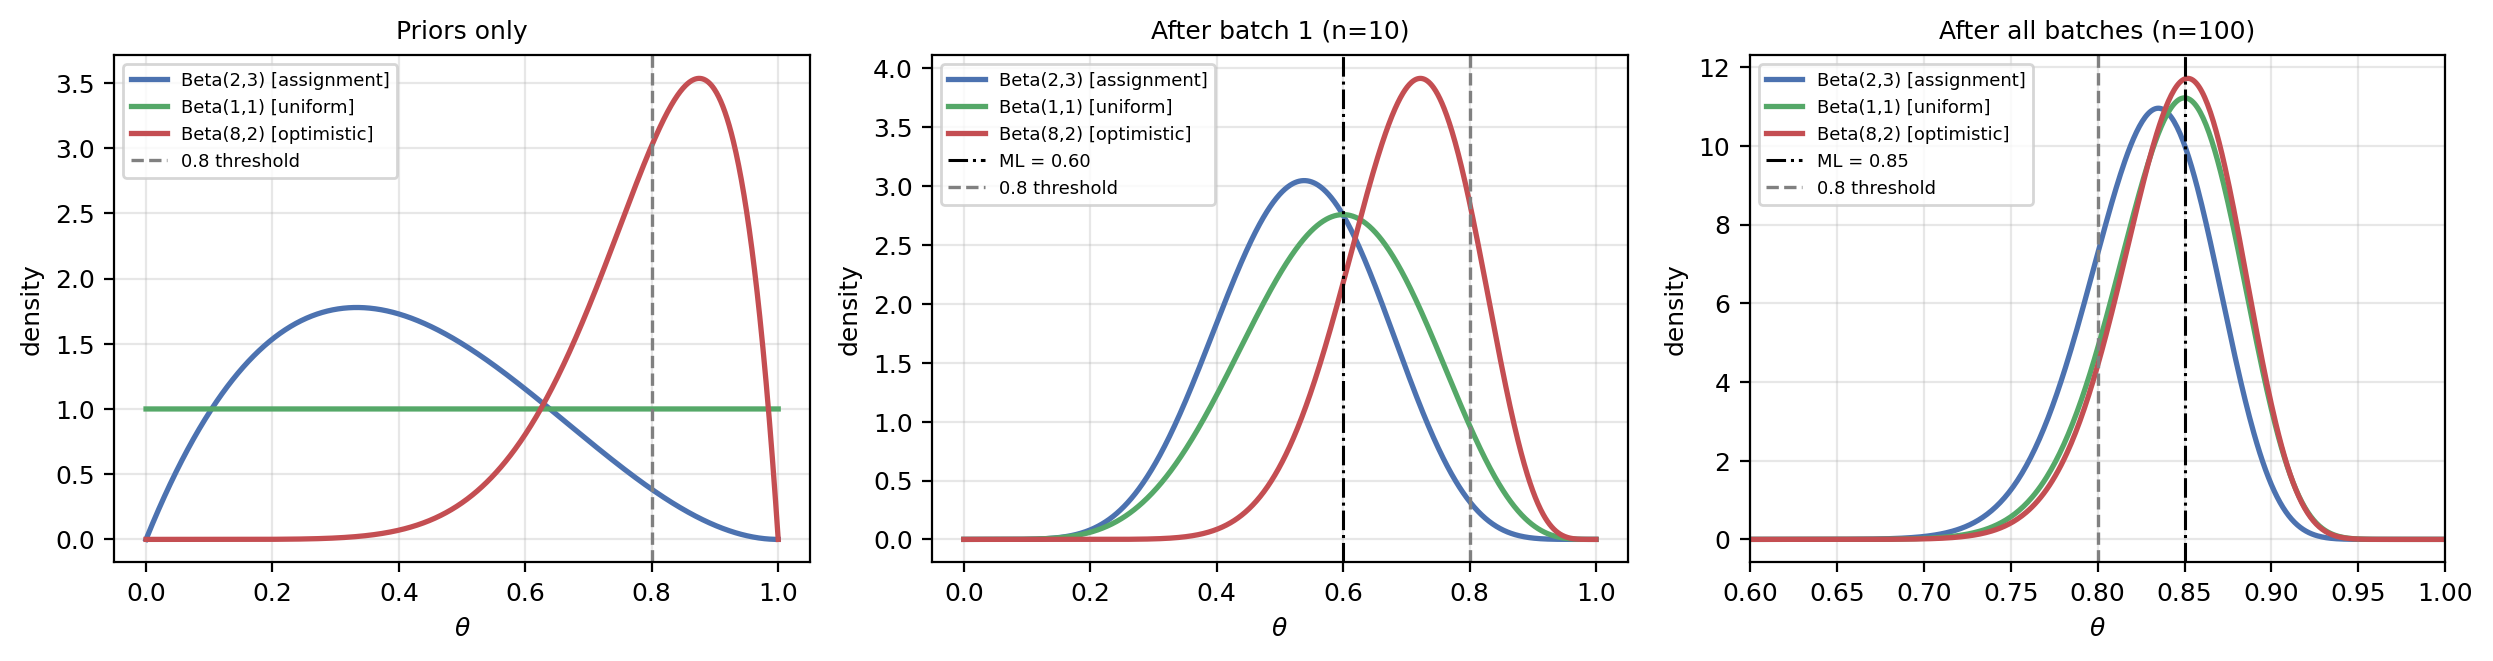
\includegraphics[width=0.495\textwidth]{../Satria_Pamungkas_21522611_COMP6010_Supplement/results/partB/B4_prior_sensitivity.png}
\caption{\textbf{Left:} sequential learning, and the final posterior with its 95\% interval and the
shaded threshold mass $P(\theta>0.8\mid\D)=0.7883$ --- visibly short of 0.95 even though the mean
exceeds 0.8. \textbf{Right:} three priors after 0, 10 and 100 attempts; the posteriors converge as
data accumulate.}
\label{fig:B}
\end{figure}

\subsection{B4. The role of the prior}

\begin{table}[H]\centering\small
\caption{Prior sensitivity. After 10 attempts the priors disagree materially; after 100 they nearly
agree. \textcolor{gray}{\small\texttt{B4\_prior\_sensitivity.csv}}}
\label{tab:Bprior}
\begin{tabular}{lccccccc}
\toprule
& \multicolumn{3}{c}{After batch 1 ($n{=}10$, ML $=0.600$)} & \multicolumn{3}{c}{After all batches ($n{=}100$, ML $=0.850$)} & \\
\cmidrule(lr){2-4}\cmidrule(lr){5-7}
Prior & Post.\ mean & MAP & $P(\theta{>}0.8)$ & Post.\ mean & MAP & $P(\theta{>}0.8)$ & Rule met? \\
\midrule
$\mathrm{Beta}(2,3)$ assignment & 0.5333 & 0.5385 & 0.0116 & 0.8286 & 0.8350 & 0.7883 & No \\
$\mathrm{Beta}(1,1)$ uniform    & 0.5833 & 0.6000 & 0.0504 & 0.8431 & 0.8500 & 0.8811 & No \\
$\mathrm{Beta}(8,2)$ optimistic & 0.7000 & 0.7222 & 0.1631 & 0.8455 & 0.8519 & 0.9009 & No \\
\bottomrule
\end{tabular}
\end{table}

After batch 1 the priors are worth 5, 2 and 10 pseudo-attempts against only 10 real ones, so the
posterior means span $0.533$--$0.700$ and the threshold probabilities differ by a factor of 14
($0.012$ to $0.163$). After 100 attempts the likelihood dominates: means collapse into
$0.829$--$0.846$, a spread of $0.017$, all near ML $=0.850$. The threshold probability stays more
prior-sensitive than the mean ($0.788$--$0.901$) because it depends on the posterior \emph{tail}
rather than its centre --- worth noting here, since a decision stated as a tail probability is more
fragile under prior choice than one stated as a point estimate. The rule fails under all three priors,
so that conclusion is robust; had it flipped, the honest reading would be that the data are too weak
to support it.

\textbf{ML and MAP under a uniform prior.} With $\mathrm{Beta}(1,1)$ the prior is constant, so it
contributes no $\theta$-dependence and maximising the posterior \emph{is} maximising the likelihood:
$\hat\theta_{\mathrm{MAP}}=\frac{(1+s)-1}{(1+s)+(1+n-s)-2}=\frac{s}{n}=\hat\theta_{\mathrm{ML}}$,
confirmed numerically at both stages ($0.600$ and $0.850$).

\textbf{Why that does not make the Bayesian answer identical to ML.} The coincidence concerns only the
single highest point of the density. Everything else differs. The posterior \emph{mean} under
$\mathrm{Beta}(1,1)$ is $(1{+}s)/(2{+}n)=0.8431$ --- Laplace smoothing, not $0.850$ --- and it is the
predictive probability for the next attempt, so even the flat-prior Bayesian \emph{prediction} differs
from the ML plug-in. More fundamentally, ML returns a number while the posterior returns a
distribution, from which credible intervals and $P(\theta>0.8\mid\D)$ follow; ML has no mechanism to
produce the quantity the deployment rule asks for. The gap matters most where decisions are riskiest:
with 5 successes in 5 attempts, ML and MAP both give $\hat\theta=1.0$ --- implying the next attempt
\emph{cannot} fail --- while the flat-prior predictive gives $0.857$ with interval $[0.541,0.996]$.
Optimising a point and carrying a distribution are different operations; only the second propagates
uncertainty into the decision.

\section{Part C (option C2): animal-drawing generation with flow matching}

\subsection{C1. Method, and the two research questions}

\textbf{Goal and data.} A class-conditional generative model over $28\times28$ grayscale line
drawings: given a requested category $y\in\{\textrm{cat},\textrm{dog},\textrm{fish}\}$ and fresh
Gaussian noise, produce a new drawing of that category. Data: Google Quick, Draw!
\texttt{numpy\_bitmap} files (CC BY 4.0, Google Creative Lab), 4{,}000 original drawings per category.

\textbf{Straight-line flow matching.} For noise $x_0\sim\mathcal{N}(0,I)$ and a real drawing
$x_1\sim p_{\text{data}}$, define the interpolation and its \emph{constant} velocity
\[
x_t=(1-t)x_0+t\,x_1,\qquad u_t=\frac{dx_t}{dt}=x_1-x_0,\qquad t\sim\mathcal{U}[0,1],
\]
and regress it with a time- and class-conditional network:
$\;\mathcal{L}_{\text{CFM}}(\theta)=\mathbb{E}_{t,x_0,(x_1,y)}\big\|v_\theta(t,x_t,y)-(x_1-x_0)\big\|^2$.
Because the path is a straight line, the target is available in closed form and \emph{no ODE is
simulated during training}. Generation integrates the learned ODE
$dx/dt=v_\theta(t,x,y)$ from $t{=}0$ to $t{=}1$.

\begin{center}\small
\begin{tabular}{@{}l@{}}
\hline
\textbf{Training} (targets known in closed form): \;
$x_0\sim\mathcal{N}(0,I)$, $x_1\sim p_{\text{data}}$, $t\sim\mathcal{U}[0,1]$
$\;\to\;x_t=(1{-}t)x_0{+}tx_1\;\to\;v_\theta(t,x_t,y)\;\xrightarrow{\ \text{MSE vs }x_1-x_0\ }\;\nabla_\theta$\\
\textbf{Generation} (integrate forward): \;
$x_0\sim\mathcal{N}(0,I)\;\to\;\big[\,x\leftarrow x+\Delta t\cdot v_\theta(t,x,y)\,\big]\times n_{\text{steps}},\; t:0\to1\;\to\;x(1)=\text{drawing}$\\
\hline
\end{tabular}
\end{center}

A single $x_t$ could have arisen from many $(x_0,x_1)$ pairs, so what does the regression learn? The
MSE-optimal prediction is the \emph{conditional mean} $\mathbb{E}[x_1-x_0\mid x_t,y]$, and it is a
theorem of flow matching that this marginal velocity field transports $\mathcal{N}(0,I)$ to
$p_{\text{data}}$ exactly. The network learns the average direction of travel, not the particular pair.

\textbf{Link to the unit.} The same three-part pattern as Parts A and B. \emph{Known structure:} the
noise distribution and the interpolation path, both chosen by me, not learned. \emph{Unknown component
learned from data:} the velocity field --- which, exactly like the quantities estimated in A and B, is
a conditional expectation. \emph{Generation by sampling:} integrate the ODE from a fresh $x_0$. The
analogy with A4 is precise: the interpolation defines a \emph{known} forward corruption
$x_1\to x_t$, but the forward process alone does not determine the reverse dynamics, because
$\mathbb{E}[x_1-x_0\mid x_t]$ depends on $p_{\text{data}}$ --- just as fixing downstream evidence in a
forward sampler does not give the posterior without a correction.

\textbf{Q1 (training factor).} Does longer training improve recognisability, and at what cost to
diversity? \emph{Predicted:} sharp gain from epoch 5 to 15, then flat; loss keeps falling; diversity
constant. \textbf{Q2 (inference factor).} How few ODE steps suffice, and does midpoint beat Euler at
matched network evaluations (NFE)? \emph{Predicted:} few steps suffice, saturating by 10--25; at
matched NFE midpoint gains little, because straight-trained paths have little curvature for a
second-order solver to exploit.

\subsection{C2. Implementation, and three key code sections}

\begin{table}[H]\centering\small
\caption{Baseline configuration. Trained entirely from scratch --- no pretrained weights, nothing
frozen. \textcolor{gray}{\small\texttt{C\_reproduction\_record.json}}}
\label{tab:Cconf}
\begin{tabular}{@{}llll@{}}
\toprule
Data & 4{,}000 orig.\ drawings/class $\times$ 3 & Architecture & \texttt{VelocityUNet} $28{\to}14{\to}7$, ch.\ $64{\to}128$ \\
Split & 9{,}600 train / 2{,}400 held out (orig.) & Trainable params & 1{,}838{,}081 (all of them) \\
Preprocessing & $[0,255]\!\to\![-1,1]$, no resize & Conditioning & sinusoidal $t$ + class embedding, per block \\
Augmentation & random h-flip, train split only & Optimiser & AdamW, lr $2\!\times\!10^{-4}$, cosine, wd $10^{-4}$ \\
Filter & ink fraction $\in[0.05,0.55]$ (8/20{,}700 rejected) & Batch / epochs & 128 / 60, grad-norm clip 1.0 \\
Seeds & split+train \texttt{20260910}; 32 generation seeds & Hardware / time & RTX 3060 (12\,GB), \textbf{6.39 min} \\
\bottomrule
\end{tabular}
\end{table}

\textbf{(a) Training examples and targets --- \texttt{flow\_matching\_batch} (\texttt{flow\_model.py}),
called in \texttt{train()}.} \emph{In:} clean drawings \texttt{x1} $(B,1,28,28)$. \emph{Out:}
\texttt{(x\_t, t, target)}. It draws Gaussian \texttt{x0} of the same shape and one uniform \texttt{t}
per image, reshaped to $(B,1,1,1)$ so it broadcasts across all pixels of that image (a per-image
scalar, not per-pixel), forms \texttt{x\_t = (1-t)*x0 + t*x1}, and returns \texttt{x1 - x0}. Each
example is a fresh $(x_0,t)$ pair, so a drawing is seen at many noise levels.

\textbf{(b) Loss and updates --- inner loop of \texttt{train()} (\texttt{train\_flow.py}).}
\emph{In:} a batch \texttt{(x1, y)}, model, optimiser. \emph{Out:} one gradient step. It applies the
flip augmentation (train split only), builds the triple, and computes
\texttt{loss = mean((model(t,x\_t,y) - target)**2)} --- this \emph{is} $\mathcal{L}_{\text{CFM}}$, with
the expectation over $t,x_0$ realised by the random batch. Then
\texttt{zero\_grad}$\to$\texttt{backward}$\to$clip$\to$\texttt{step}. The whole generative model
reduces to a regression. \texttt{eval\_loss} measures held-out loss over a \emph{fixed} grid of $t$ so
checkpoints are comparable rather than differing by sampling noise.

\textbf{(c) Generation --- \texttt{sample\_ode} (\texttt{flow\_model.py}).} \emph{In:} model, count,
labels, \texttt{n\_steps}, \texttt{method}, \texttt{seed}. \emph{Out:} images, \textbf{NFE}, optional
trajectory. It seeds a generator, draws $x_0$ --- \emph{the only randomness} --- and steps $t:0\to1$.
Euler uses one network evaluation per step; midpoint two. NFE is returned explicitly because
comparing solvers at matched \emph{step count} would silently give midpoint double the compute.

\textbf{Verification before training.} I asserted the shapes match, that \emph{all} parameter tensors
receive non-zero gradient, and specifically that \texttt{class\_embed.weight.grad} is non-zero --- a
dead conditioning path fails silently, since the loss still falls while every class generates the same
thing. Endpoint checks confirmed $\max|x_t-x_0|$ at $t{=}0$ and $\max|x_t-x_1|$ at $t{=}1$ are
${\sim}10^{-7}$.

\begin{figure}[H]\centering
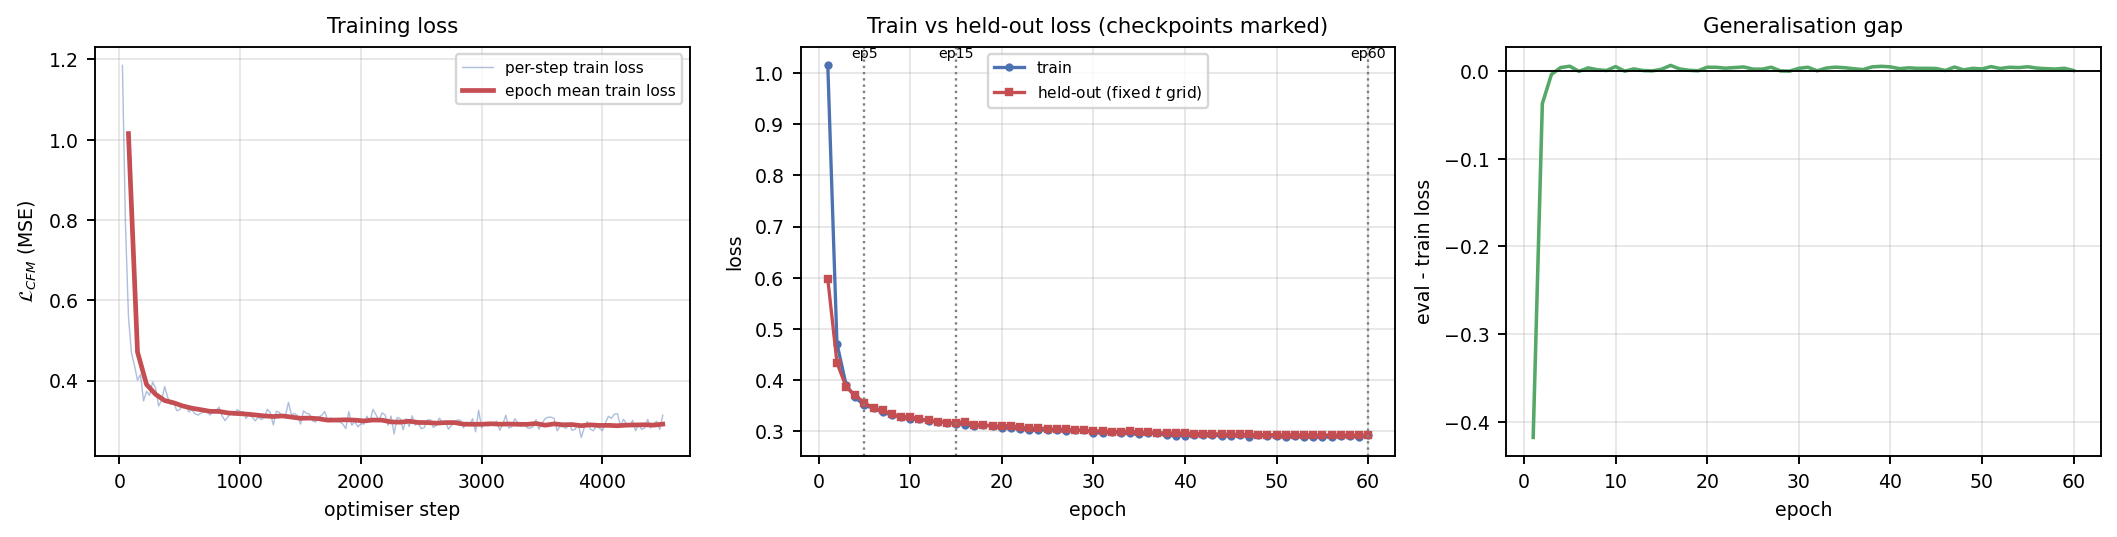
\includegraphics[width=0.60\textwidth]{../Satria_Pamungkas_21522611_COMP6010_Supplement/results/partC/C_training_curves.png}
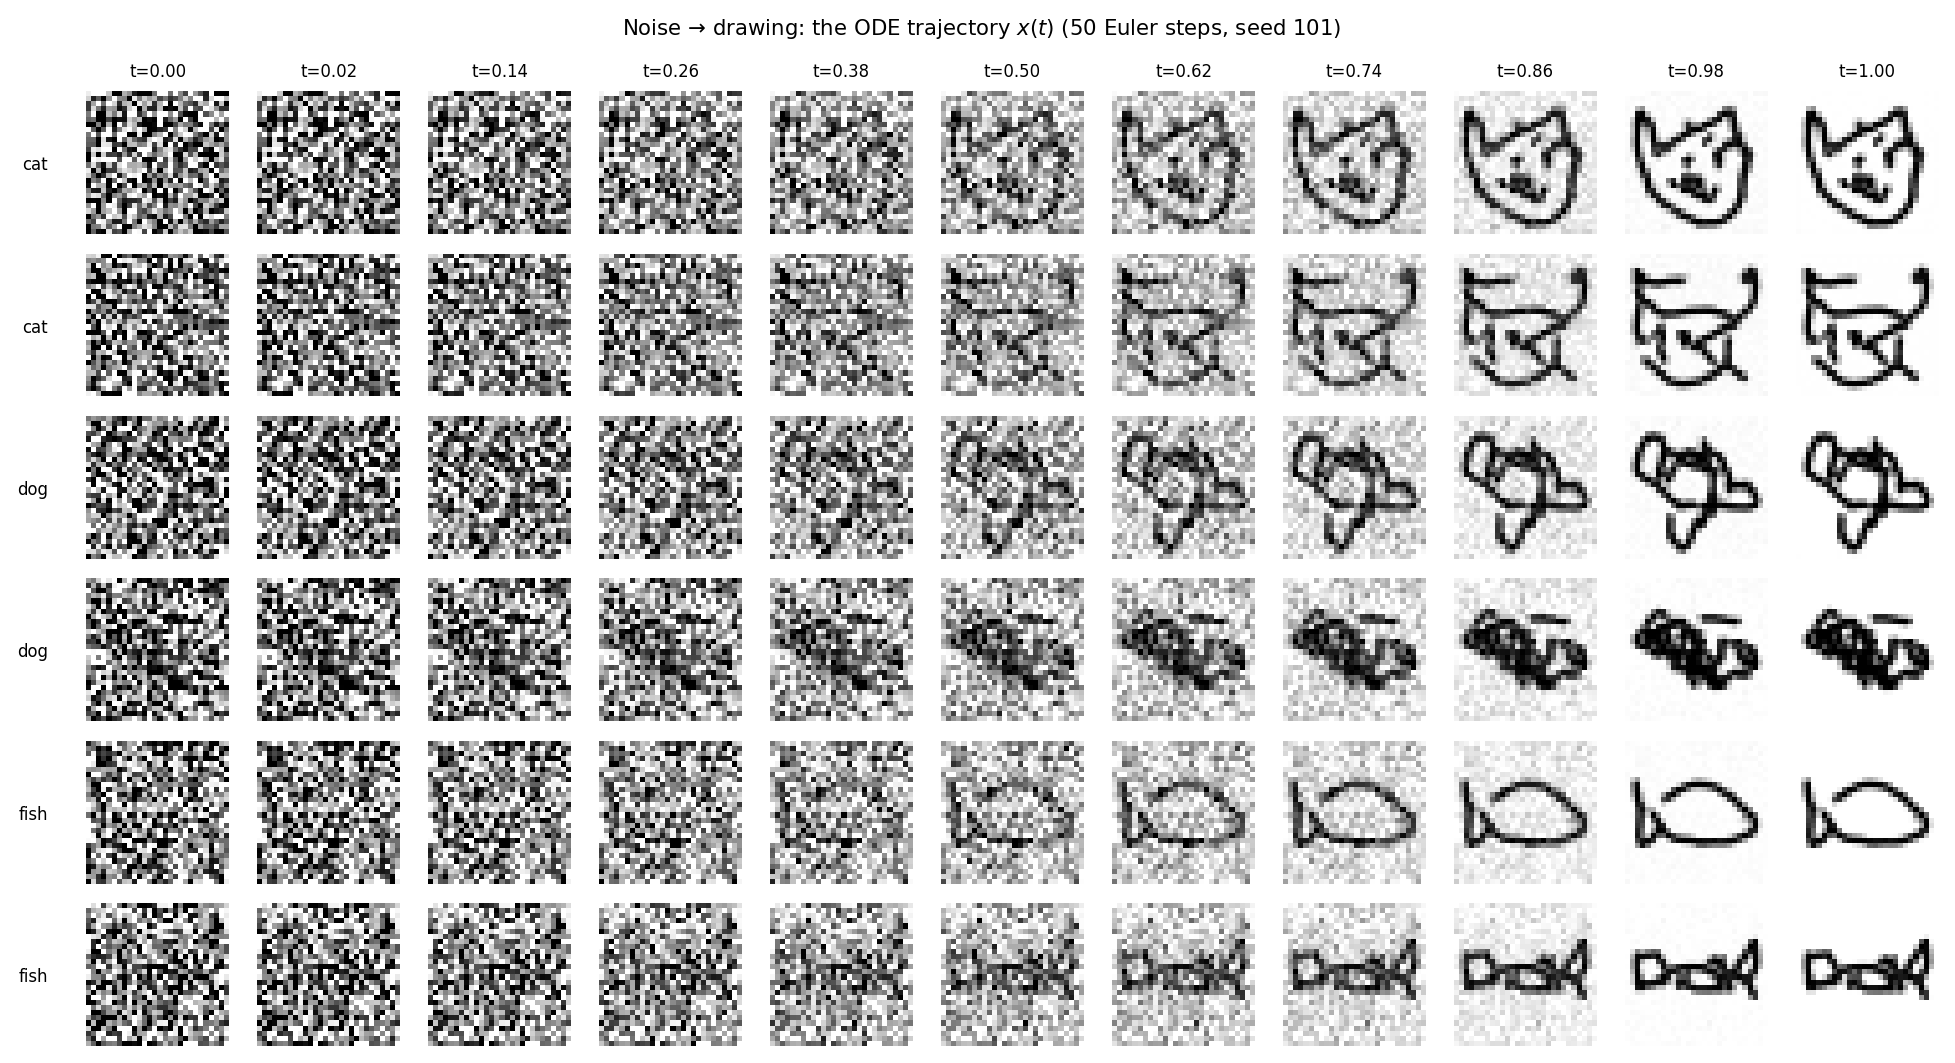
\includegraphics[width=0.385\textwidth]{../Satria_Pamungkas_21522611_COMP6010_Supplement/results/partC/C_trajectory_noise_to_drawing.png}
\caption{\textbf{Left:} training and held-out loss (checkpoints marked). Held-out loss never exceeds
train loss by more than $0.006$ --- no overfitting at this size. \textbf{Right:} the ODE trajectory
$x(t)$ from noise to drawing; broad structure appears by $t{\approx}0.3$--$0.5$ and later steps sharpen
strokes, consistent with near-straight paths.
\textcolor{gray}{\small\texttt{C\_training\_curves.png}, \texttt{C\_trajectory\_noise\_to\_drawing.png}}}
\label{fig:Ctrain}
\end{figure}

\subsection{C3--C4. Controlled comparisons and evaluation}

\textbf{Protocol.} A predetermined list of \textbf{32 seeds}, fixed once and reused in \emph{every}
comparison; each seed gives one sample per class, so \textbf{96 outputs per configuration} (32 per
class, against the required minimum of 16 total and 4 per class). I exceed the minimum deliberately:
a first run with 8 seeds (24 outputs) returned an identical $0.75$ for all three checkpoints, a
discretisation artefact rather than a finding. One factor changes at a time; data and evaluation inputs
are fixed. \textbf{Quality measure:} \emph{recognisability} --- the fraction of a configuration's full
96-sample set that an independent CNN assigns to the \emph{requested} class. That CNN is trained
\emph{only on real held-out drawings}, data the generator never saw, and it scores \textbf{0.8375} on
real held-out drawings --- so $0.8375$, not $1.0$, is the ceiling.

\begin{table}[H]\centering\small
\caption{Both comparisons. Binomial standard error is $\pm0.041$ throughout ($n{=}96$), so differences
below ${\sim}0.09$ are not resolvable. \textcolor{gray}{\small\texttt{C\_all\_results.csv}}}
\label{tab:Cres}
\begin{tabular}{@{}llrrrrrr@{}}
\toprule
& Config & Held-out loss & Recog.\ ($\pm$0.041) & Confidence & Diversity & NFE/img & ms/img \\
\midrule
\multirow{4}{*}{\rotatebox{90}{\scriptsize training}}
& epoch 5   & 0.3557 & 0.781 & 0.637 & 22.6 & 50 & 16.3 \\
& epoch 15  & 0.3164 & 0.771 & 0.672 & 22.1 & 50 & 16.3 \\
& epoch 60 (baseline) & 0.2922 & \textbf{0.802} & \textbf{0.704} & 22.5 & 50 & 16.3 \\
& epoch 60, \emph{quarter} data & 0.3297 & 0.760 & --- & 22.1 & 50 & 16.3 \\
\midrule
\multirow{6}{*}{\rotatebox{90}{\scriptsize inference}}
& Euler 2 steps    & --- & 0.781 & 0.630 & \textbf{14.9} & 2 & 0.76 \\
& Euler 5 steps    & --- & 0.792 & 0.703 & 20.6 & 5 & 1.74 \\
& Euler 10 steps   & --- & 0.792 & 0.706 & 21.7 & 10 & 3.35 \\
& Euler 50 steps   & --- & 0.802 & 0.704 & 22.5 & 50 & 16.3 \\
& Euler 100 steps  & --- & 0.792 & 0.702 & 22.6 & 100 & 32.1 \\
& Midpoint 5 steps & --- & 0.802 & 0.707 & 22.7 & 10 & 3.32 \\
\bottomrule
\end{tabular}
\end{table}

\begin{figure}[H]\centering
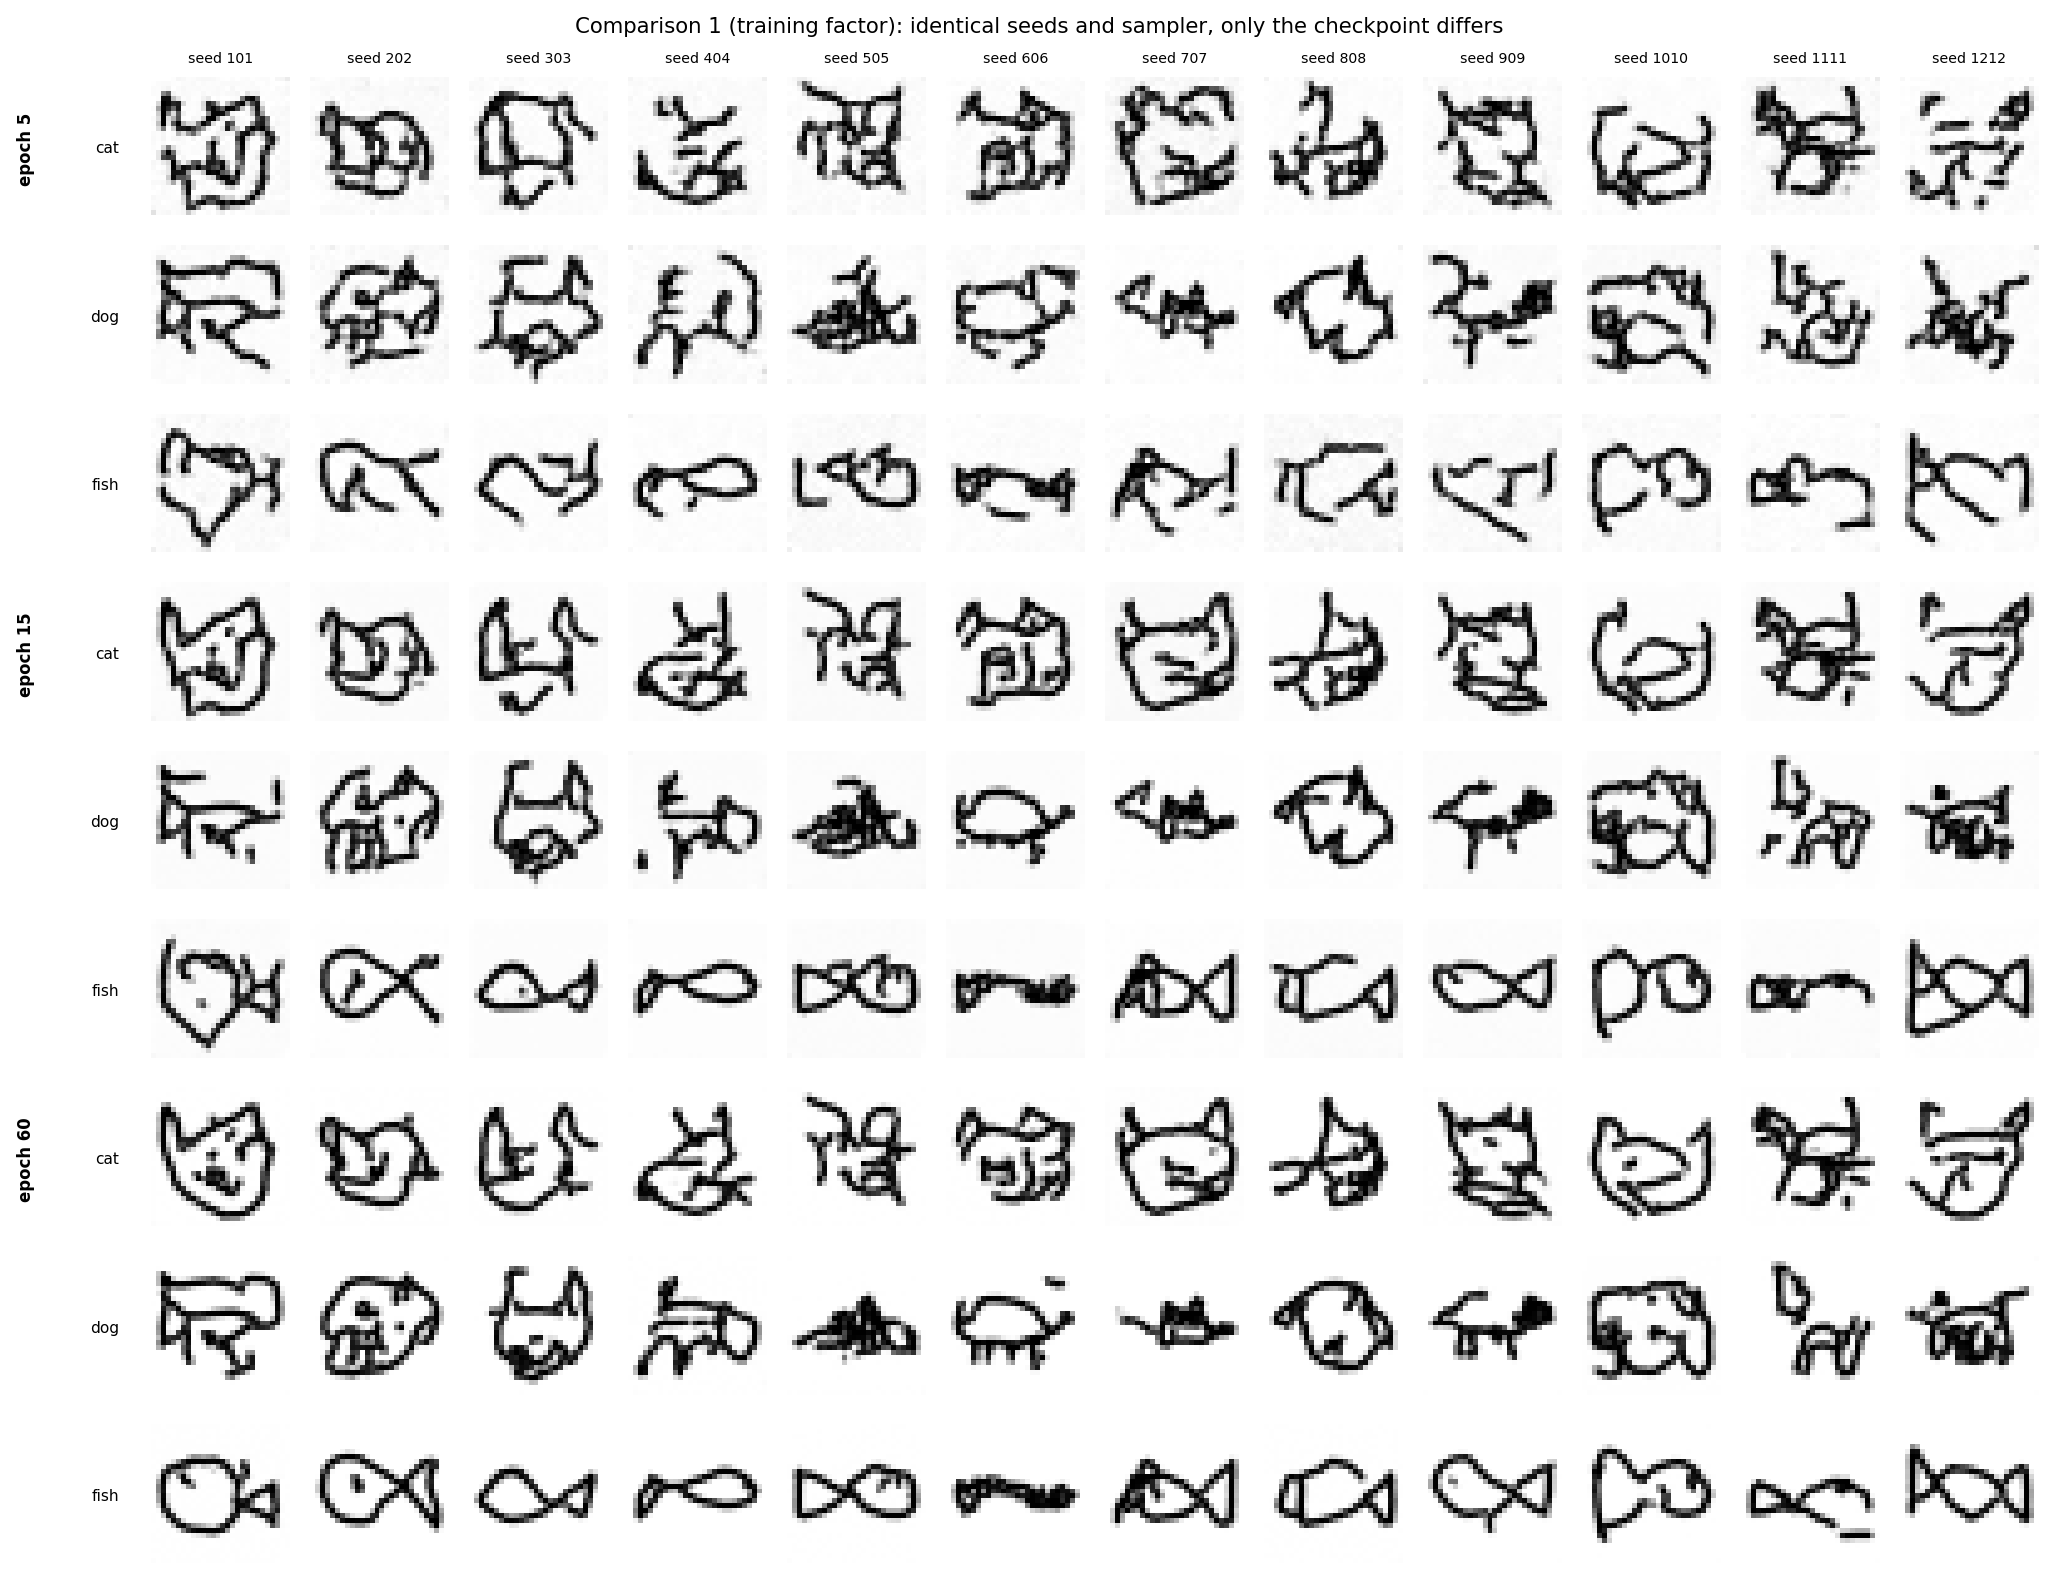
\includegraphics[width=0.485\textwidth]{../Satria_Pamungkas_21522611_COMP6010_Supplement/results/partC/C_matched_grid_checkpoints.png}
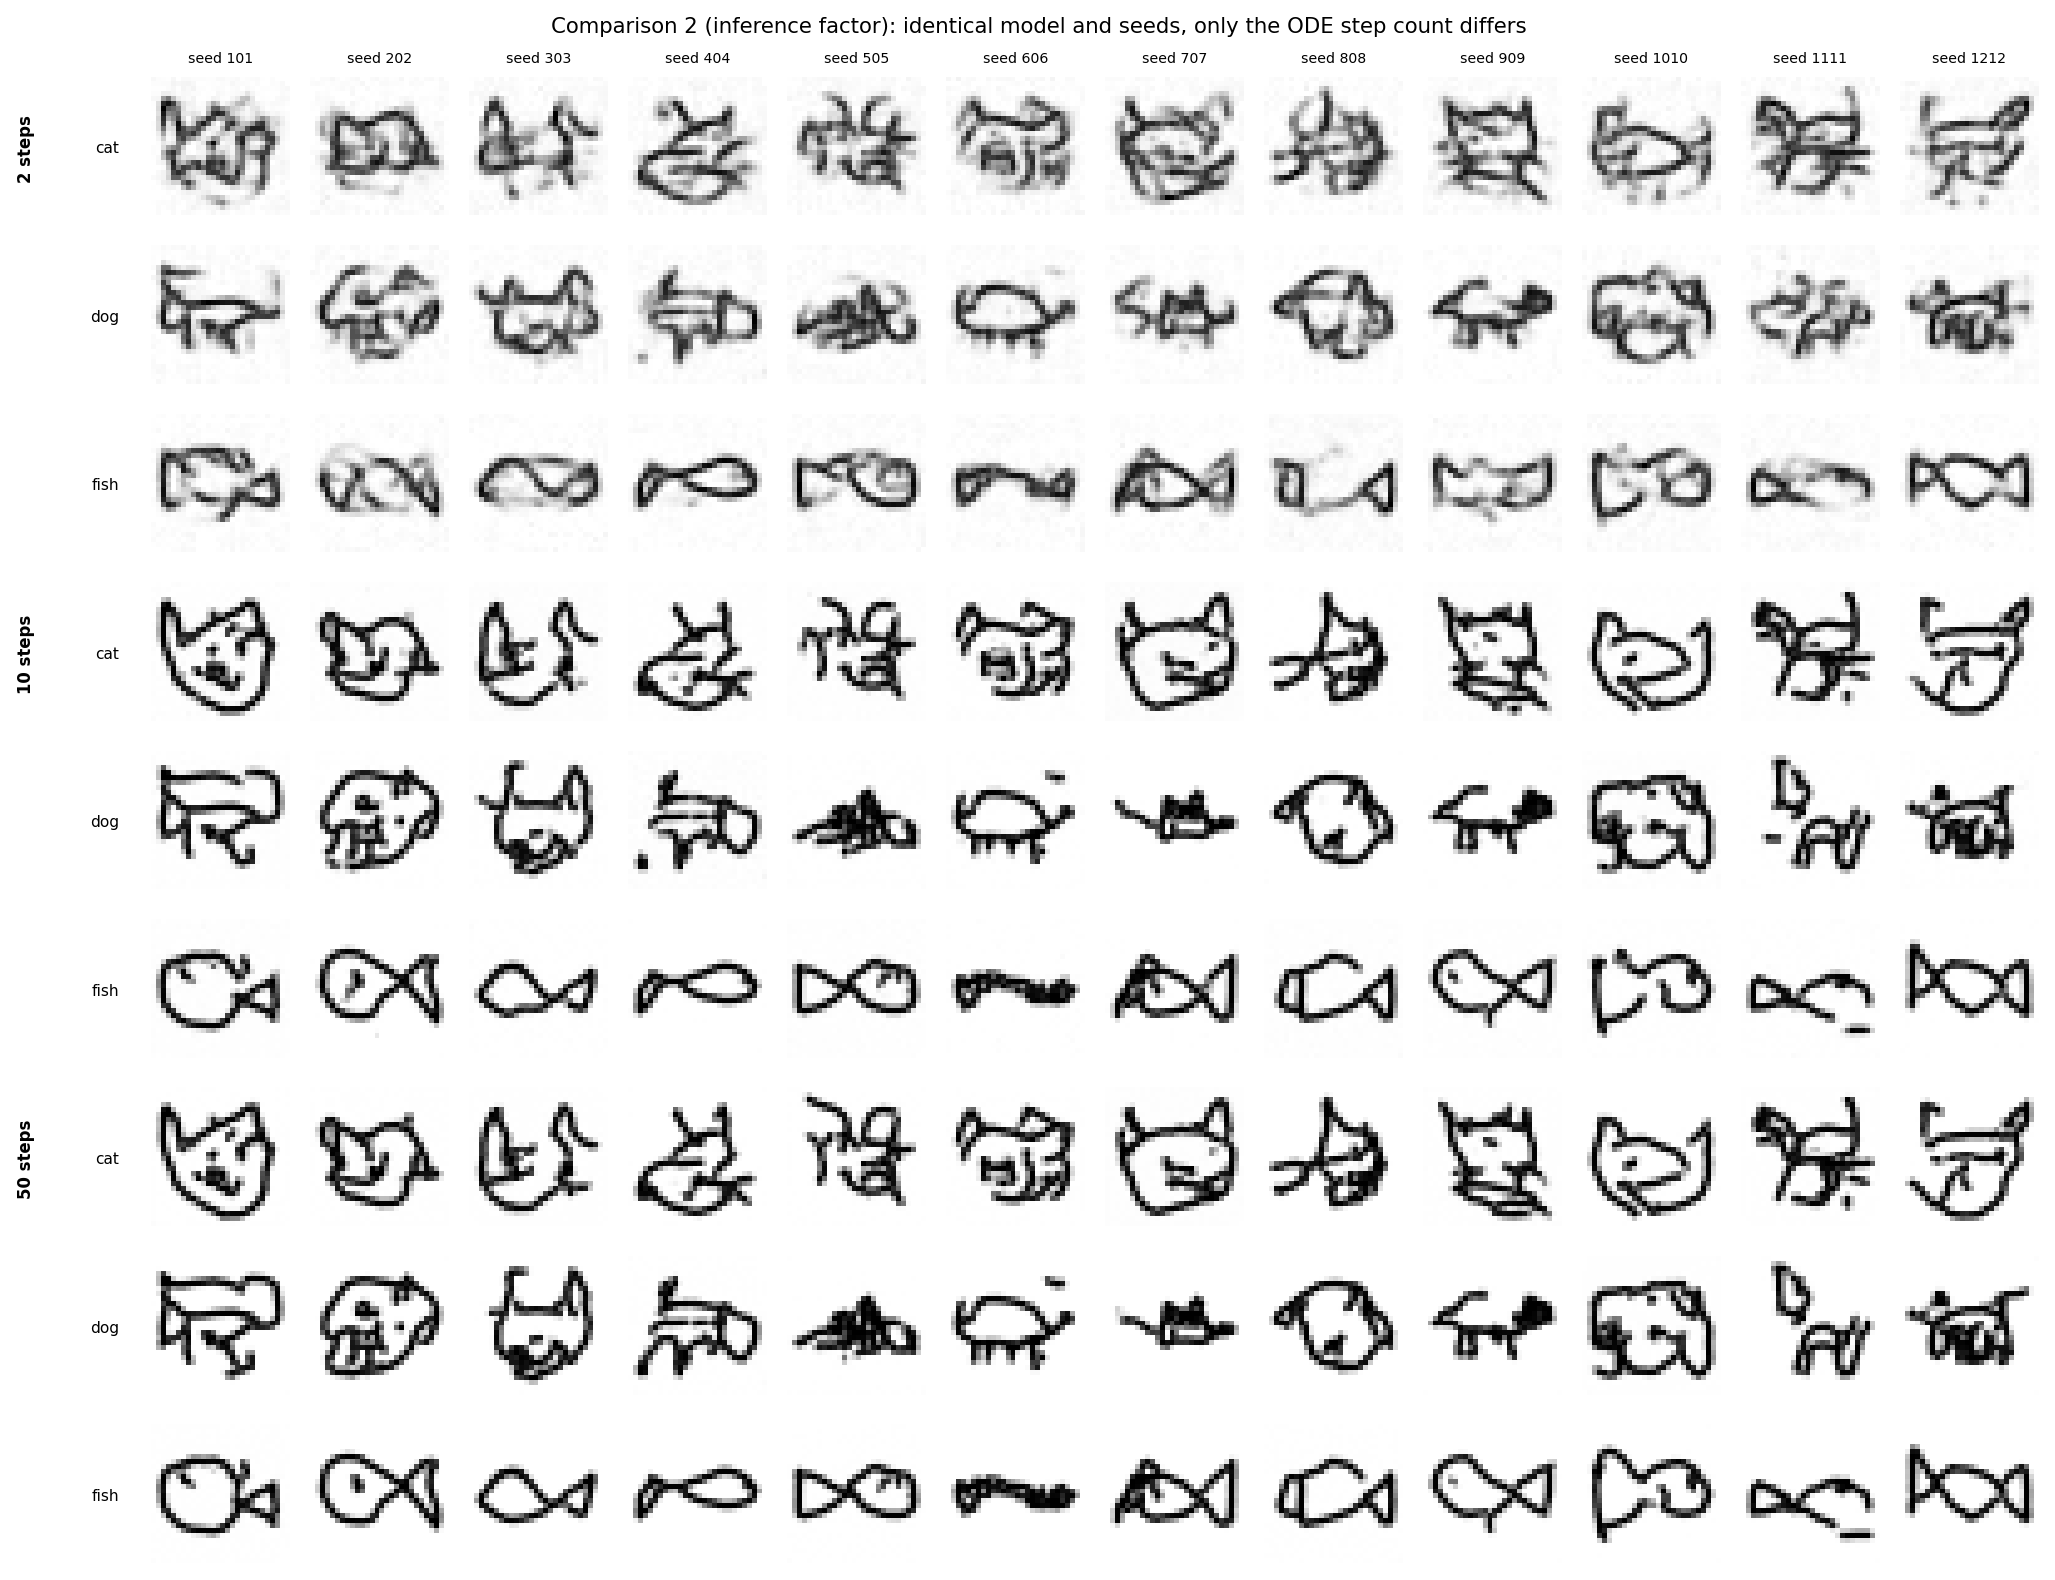
\includegraphics[width=0.485\textwidth]{../Satria_Pamungkas_21522611_COMP6010_Supplement/results/partC/C_matched_grid_steps.png}
\caption{Matched grids, identical seeds down the columns, first 12 of 32 seeds shown; failures
included. \textbf{Left (Q1):} only the checkpoint differs. Visual quality clearly improves --- epoch-5
cats are scribbly, epoch-60 cats have clean ears and faces, epoch-60 fish are crisp --- even though the
recognisability \emph{metric} moved within noise. \textbf{Right (Q2):} only the ODE step count differs;
the 2-step row is visibly faint and washed out, while 10 and 50 steps are near-indistinguishable.
Complete 96-sample sets for all 14 configurations, including \texttt{.npz} arrays, are in
\textcolor{gray}{\small\texttt{results/partC/sample\_grids/}}.}
\label{fig:Cgrids}
\end{figure}

\subsection{C5. Interpretation}

\textbf{Q1: my prediction was wrong, and how it is wrong is the main result.} Held-out loss fell
monotonically by 18\% (0.356$\to$0.292) and mean confidence rose steadily (0.637$\to$0.704), but
\emph{recognisability barely moved}: 0.781$\to$0.771$\to$0.802, a change of half a standard error. I
cannot claim a real accuracy gain from training 12$\times$ longer. Three conclusions follow.
\emph{First}, this is a direct quantitative demonstration that \textbf{training loss is not a measure
of generated-image quality} --- loss improved 18\% while the sample-level score stayed within noise,
because the CFM loss averages velocity error over all $t$ and most residual reduction happens at noise
levels that barely affect where the trajectory lands. \emph{Second}, confidence was the more sensitive
instrument: the thresholded arg-max decision discards information that longer training genuinely
improved, so reporting accuracy alone would have hidden a real effect --- while reporting it \emph{as
if} it showed one would have invented an effect. \emph{Third}, the task saturates almost immediately:
by epoch 5 (32 seconds) samples already score 0.781 against a ceiling of 0.8375, leaving little
headroom. Crucially, the grids in Fig.~\ref{fig:Cgrids} show that visual quality \emph{does} improve
substantially --- so the honest conclusion is that my \emph{metric} was too coarse for this factor,
not that training does nothing. Per-class results locate the difficulty: \texttt{fish} scores
0.94--0.97 at every checkpoint while \texttt{dog} scores 0.53--0.66, mirroring the classifier's own
real-data ceilings (fish 0.916, cat 0.821, dog 0.781) --- dogs are the hardest class in this dataset
for evaluator and generator alike, so this reflects the data, not broken conditioning. The
\emph{dataset-size} comparison is the training factor that does move: quartering the data at identical
optimisation budget raises held-out loss 0.292$\to$0.330 and lowers recognisability 0.802$\to$0.760.
At this model size the binding constraint is data, not steps.

\textbf{Q2: both halves of the prediction hold, and saturation is more extreme than predicted.}
Recognisability is flat from 2 to 100 Euler steps --- all within one standard error. What \emph{does}
change at 2 steps is \textbf{diversity}, collapsing from ${\sim}22.5$ to $\mathbf{14.9}$ (a 34\% drop,
far outside the variability elsewhere), with confidence also falling to 0.630. The 2-step failure mode
is therefore not ``wrong class'' but ``under-integrated'': samples land in roughly the right region yet
are washed-out and mutually similar, exactly as Fig.~\ref{fig:Cgrids} (right) shows. Beyond ${\sim}5$
steps extra steps buy nothing measurable while cost grows linearly --- 0.76\,ms to 32.1\,ms per image
from 2 to 100 steps, a 42$\times$ increase for no measurable gain. This is flow matching's practical
appeal over DDPM sampling: straight-line targets give near-straight trajectories, so a handful of steps
suffices where diffusion typically needs hundreds. At \textbf{matched NFE} the Euler/midpoint
differences are $+0.010$, $-0.010$ and $0.000$, each far below the $\pm0.058$ standard error of the
difference, so no configuration is distinguishable --- matching the geometric argument that a
second-order solver's advantage scales with curvature. Midpoint's only visible edge is at the very
lowest budget: at NFE 4 it recovers diversity 23.7 against Euler's 14.9 at NFE 2.
\textcolor{gray}{\small\texttt{C\_comparison2\_matched\_nfe.csv}}

\textbf{Why generation is random although the solver is deterministic.} Both solvers are deterministic
maps --- fixing $x_0$ fixes the output exactly, which is what makes the 32-seed list reproducible. I
verified this rather than assuming it, and the check caught something worth recording: with default
settings two runs of the \emph{same} seed differed by ${\sim}7\times10^{-4}$, because cuDNN is free to
choose non-deterministic convolution algorithms and TF32 reductions. The mathematics was never the
problem --- $x_0$ was bitwise identical --- but the claim ``the same seed reproduces the same image''
was only true to plotting precision until I pinned the backend (\texttt{enable\_deterministic()} in
\texttt{flow\_model.py}), after which same-seed runs are bitwise equal and the notebook asserts it. All
randomness enters through the \emph{initial condition} $x_0\sim\mathcal{N}(0,I)$; the ODE
deterministically transports the noise distribution onto the data distribution. Variety comes from
where you start, not from noise injected en route --- the structural difference from a stochastic
diffusion sampler.

\textbf{Memorisation.} Mean $L_2$ distance from each of the 96 generated samples to its nearest
\emph{training} drawing is \textbf{16.62}, against \textbf{15.69} for 200 real \emph{held-out} drawings
measured the same way. Generated samples are thus \emph{further} from the training set than genuinely
unseen real drawings are --- evidence against wholesale copying. Inspecting the six closest pairs, they
share only coarse layout (a body outline, a tail direction), not stroke-for-stroke identity. Resemblance
alone is not proof: with 3{,}200 training drawings per class of simple doodles, any plausible new cat
\emph{must} resemble some training cat, so the distance \emph{distribution} is the meaningful comparison,
not any single pair. \textcolor{gray}{\small\texttt{C\_memorisation\_distances.csv}, \texttt{C\_memorisation\_probe.png}}

\textbf{Limitations of the measure, and of the study.}
(i) The ceiling is $0.8375$, not $1.0$, because Quick, Draw! doodles are genuinely ambiguous; epoch 60
reaches 96\% of it. (ii) The classifier is an imperfect proxy with its own biases --- a high score is
necessary but not sufficient for ``a human would call this a cat''. (iii) \textbf{It measures
conditioning, not fidelity, and this bit me}: the 2-step samples scored 0.781, statistically
indistinguishable from 50 steps, despite being obviously worse and showing a 34\% diversity collapse.
Class accuracy was nearly blind to the largest quality difference in the study. (iv) At $n{=}96$ the
standard error is $0.041$, so sub-$0.09$ differences are unresolvable; only two effects in this study
exceed noise --- the 2-step diversity collapse and the quarter-data loss degradation. The rest are null
results, and detecting smaller effects would need several hundred samples per configuration (affordable
at 17\,ms/image, and the first thing I would change). (v) $L_2$ nearest-neighbour distance is a weak
perceptual metric: adequate for near-duplicate detection, blind to a semantically memorised drawing
shifted by a few pixels. (vi) $28\times28$ line drawings are the easy end of image generation; nothing
here shows the approach scales to photographs. No FID or human study --- both need far more samples or
a pretrained feature extractor, and I report only measures I can define and defend at this scale.

\section{Conclusion: inference $\rightarrow$ learning $\rightarrow$ generation}

Part~A took a \emph{fully known} model and did inference by sampling, where the entire difficulty was
conditioning on evidence correctly --- overwriting downstream evidence returned the prior ($0.0799$ vs
$q_2=0.2933$), and rejection and likelihood weighting are the two valid corrections. Part~B kept the
structure known but made \emph{one scalar} unknown, and learning a posterior over it changed the
decision: ML $=0.850$ sits above the threshold, yet $P(\theta>0.8\mid\D)=0.788$ fails the $0.95$ rule,
because a point estimate discards the width that the rule is explicitly about. Part~C makes the unknown
a \emph{function}: the noise distribution and interpolation path are chosen by me, and the velocity
field --- a conditional expectation, exactly like the quantities estimated in A and B --- is learned from
data; generation is then sampling in the same sense, pushing a draw from a known distribution through a
learned map. The through-line is that a generative model is not a different \emph{kind} of object from a
Bayesian network: it is the same factorise--learn--sample pattern with a neural network standing in for
a CPT, and the same warning holds at every scale --- a known forward process never hands you the reverse
one for free. Part~C also delivered the methodological lesson the brief anticipates: an 18\% improvement
in training loss produced no measurable change in sample quality, so the measure you choose determines
what you are able to conclude.

\section*{AI-use statement}

I used Claude (Anthropic), model Opus 5, via the Claude Code CLI on 9--10 September 2026, for
explanation of flow matching for images, code scaffolding for the U-Net and sampler, notebook structure
and debugging. All mathematical reasoning, experimental design, verification and claims are my own, and
every number reported was produced by code I ran on my own hardware. Five interactions are documented
in \texttt{AI\_USE\_LOG.md} with prompt, response excerpt, my check and the resulting decision,
including one independently verified correctness check (I re-derived Part~A's exact values with a
separate brute-force enumeration agreeing to 10 decimal places, and added a transposed-CPT test the
assistant had not suggested, showing the normalisation check is weaker than it looks) and one
prediction-versus-observation comparison (the Euler/midpoint expectation above, which the data
contradicted). I also record one suggestion I \textbf{rejected}: proposed ink-filter thresholds of
$[0.02,0.60]$ rejected \emph{nothing} when I measured the actual distribution, so I recalibrated to
$[0.05,0.55]$ rather than disclose a filter that did not filter. The log's summary table lists all 14
independent checks I ran. No result, runtime, citation or figure in this submission was fabricated.

\begin{figure}[H]\centering
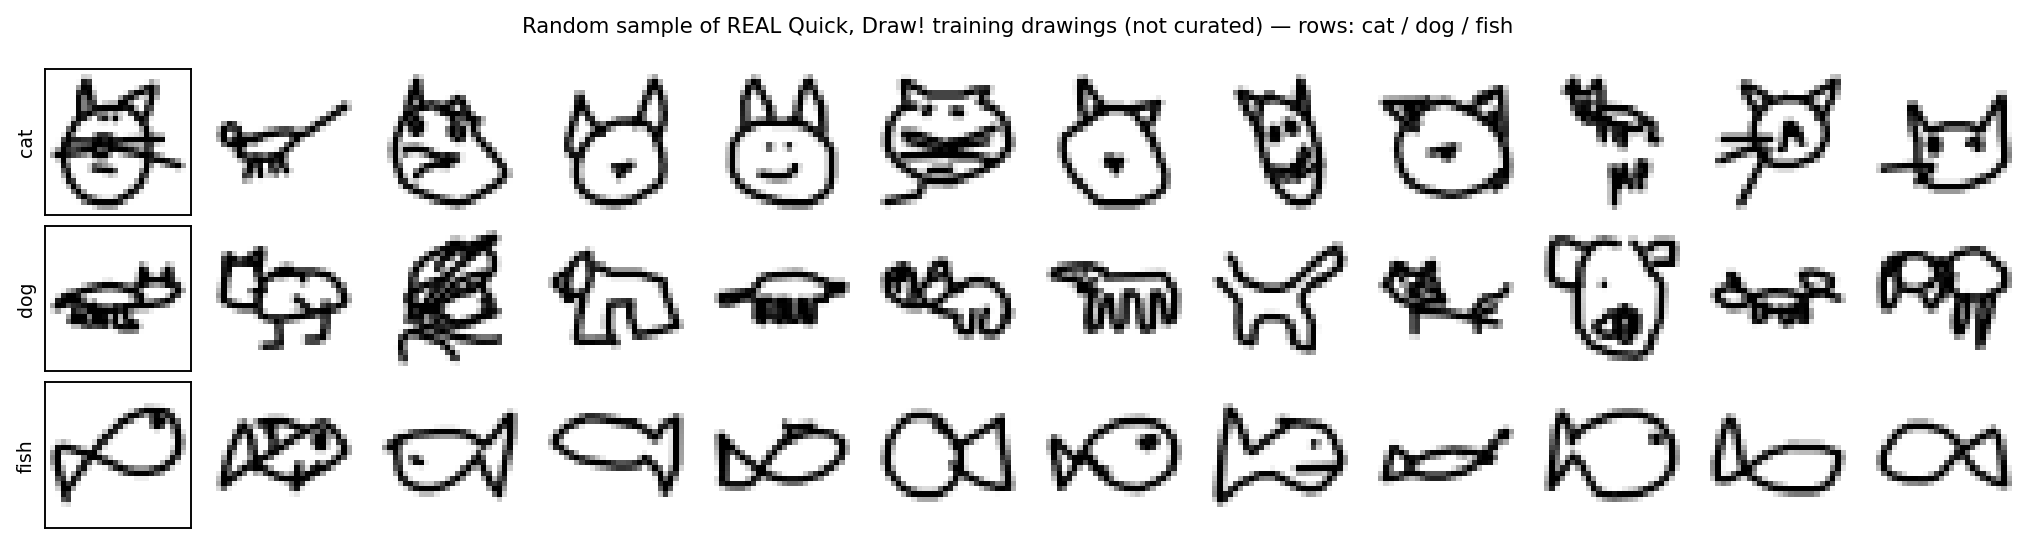
\includegraphics[width=0.615\textwidth]{../Satria_Pamungkas_21522611_COMP6010_Supplement/results/partC/C_real_data_grid.png}
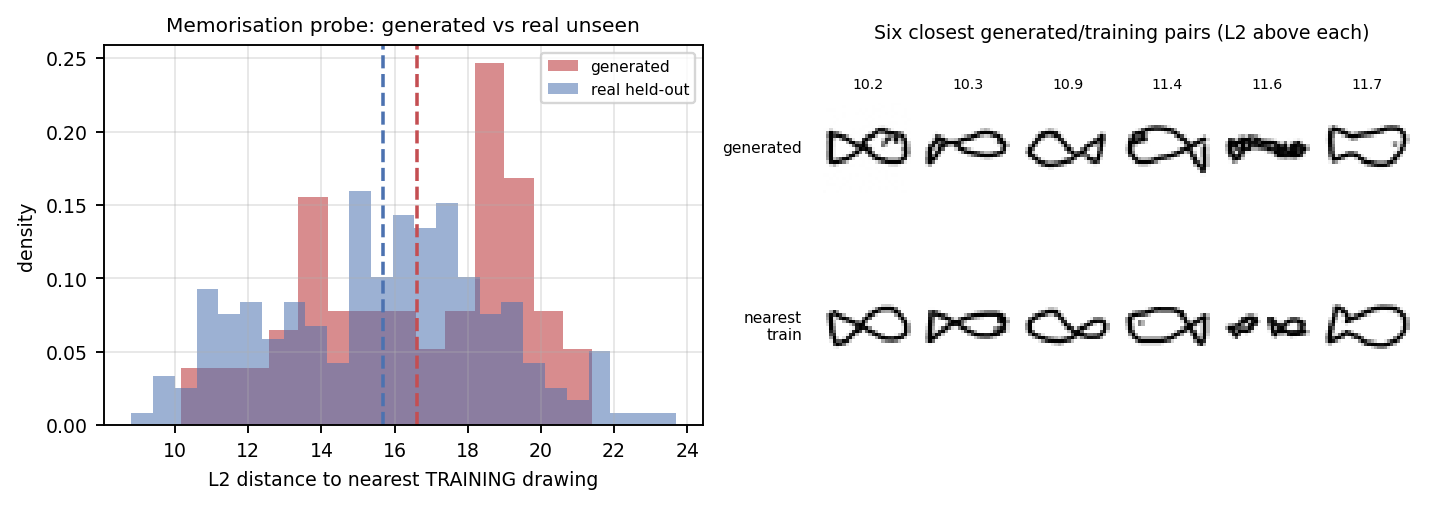
\includegraphics[width=0.375\textwidth]{../Satria_Pamungkas_21522611_COMP6010_Supplement/results/partC/C_memorisation_probe.png}
\caption{\textbf{Left:} a random (not curated) sample of the real Quick, Draw! \emph{training}
drawings, inspected before training. Several are ambiguous even to a human --- these are 20-second
public doodles --- which is what sets the $0.8375$ recognisability ceiling rather than $1.0$.
\textbf{Right:} the memorisation probe. Generated samples sit at mean $L_2$ $16.62$ from their nearest
training drawing versus $15.69$ for real held-out drawings, and even the six closest pairs share only
coarse layout, not strokes. \textcolor{gray}{\small\texttt{C\_real\_data\_grid.png}, \texttt{C\_memorisation\_probe.png}}}
\label{fig:Cdata}
\end{figure}

\section*{References}
\small
\begin{enumerate}[leftmargin=1.4em,itemsep=0pt]
\item COMP6010 teaching materials (2026): \emph{Bayesian Networks I}; \emph{Bayesian Networks 2 --
Inference}; \emph{Learning Probabilistic Models}; \emph{Diffusion and Flow Matching Models};
continuous-probability notes; Practicals 1--4, 6 and 7. Used as the primary source for all three parts.
\item Google Creative Lab. \emph{The Quick, Draw! Dataset} (\texttt{numpy\_bitmap} format), CC BY 4.0.
\url{https://github.com/googlecreativelab/quickdraw-dataset}. Categories \texttt{cat}, \texttt{dog},
\texttt{fish} retrieved 10 September 2026; SHA-256 checksums in \texttt{C\_data\_manifest.json}.
\item SciPy documentation, \texttt{scipy.stats.beta} (v1.15.3) --- Beta densities, CDF/survival
functions, quantiles and sampling. \url{https://docs.scipy.org/doc/scipy/reference/generated/scipy.stats.beta.html}
\item Lipman, Y., Chen, R.T.Q., Ben-Hamu, H., Nickel, M., Le, M. (2023). Flow Matching for Generative
Modelling. \emph{ICLR}. \url{https://arxiv.org/abs/2210.02747}
\item Liu, X., Gong, C., Liu, Q. (2023). Flow Straight and Fast: Learning to Generate and Transfer Data
with Rectified Flow. \emph{ICLR}. \url{https://arxiv.org/abs/2209.03003}
\item Meta AI. \emph{flow\_matching} library and example notebooks (adapted conceptually for the 2-D
starting point in Practical 7). \url{https://github.com/facebookresearch/flow_matching}
\item Ho, J., Jain, A., Abbeel, P. (2020). Denoising Diffusion Probabilistic Models. \emph{NeurIPS}.
\url{https://arxiv.org/abs/2006.11239} --- used for the contrast with stochastic samplers in \S C5.
\item Paszke, A.\ et al.\ (2019). PyTorch (v2.10.0+cu128). \url{https://pytorch.org}
\item Kish, L. (1965). \emph{Survey Sampling}. Wiley --- effective sample size used in \S A4.
\end{enumerate}

\end{document}
